\subsection{Composition Concepts}

The major challenge during the development of a \ms{} application is to achieve
loose coupling according to the IDEAL tenet. The goal of loose coupling is to
reduce dependencies among services. It has to be noticed that the coupling
between services can never be zero. Without any coupling the application cannot
function as a whole. MicroNet several basic concepts to reduce service coupling
while preserving reasonable development comfort. These concepts are discussed in
this section.

\subsubsection{Dependency Abstraction}

Dependency abstraction is a concept to reduce the number of dependencies
that \mss{} must explicitly add to the Java classpath to access core
functionality networking, persistence, and serialization.

According to the dependency abstraction concept external libraries are wrapped
within the core framework to offer standard access to the underlying dependency.
\mss{} can use the MicroNet wrapper libraries instead of using the
dependencies directly. This allows for exchangeability of the dependencies
without touching any \mss{} services. MicroNet integrates dependent libraries
into the wrapper libraries by the use of Maven which allows a very flexible
dependency chain. \autoref{fig:dependency_abstraction} shows which libraries are
abstracted by which framework component.

\begin{figure}
	\centering
	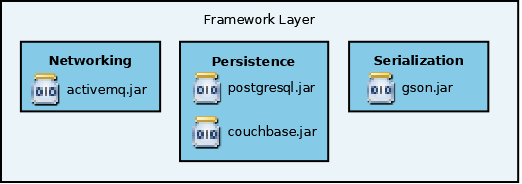
\includegraphics[width=10cm]{images/architecture/DependencyAbstraction}
	\caption{Dependency Abstraction in the MicroNet core framework.}
	\label{fig:dependency_abstraction}
\end{figure}

It has to be mentioned that the dependency abstraction layer is a dependency
itself and therefore it increases service coupling. But since the abstraction
layer unifies dependency access it helps to respect the don't repeat yourself (DRY)
principle and therefore increases overall cohesion of the application. 

Since the MicroNet adaption layer is realized using Java wrapper libraries,
this approach works very well for all Java \mss{} but none Java services have to
use the dependencies directly.

\subsubsection{Shared Model}
\label{subsub:shared_model}

The general design of how to incorporate a game model into a \mn{} application
is reclined to the design of modern game engines like Unity3D or UnrealEngine 4.
What these engines have in common is a graph to store the game state e.g. all
objects, levels, players, etc. This concept of game data organization will be
referred as the game graph. Two examples of game graphs are shown in
\autoref{fig:scenegraph}.

\begin{figure}
  \centering
  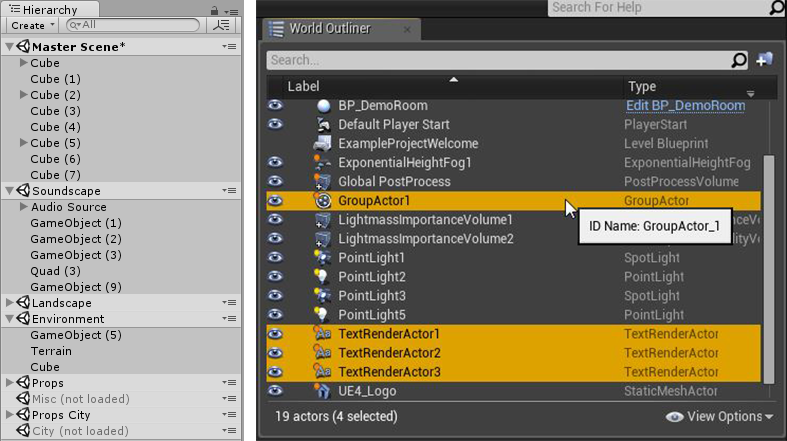
\includegraphics[width=\textwidth]{images/game_engine/scenegraph}
  \caption{Two example game graphs of the Unity3D (left) and the UnrealEngine4
  (right).}
  \label{fig:scenegraph}
\end{figure}

The shared model concept is mainly inspired by game graph concept of game
engines. The graph is represented by a Json document structure and can be shared
either using a git repository or by using a development database. The Json
format helps to achieve platform independence.

The shared model specifically allows to strongly type message transfers and
unifies database access. The design of the shared model allows to integrate the
game graph in a game engine because the concepts are closely related.

The shard model represents the game graph in the form of two individual trees:
The template tree and the prefab tree. The template tree is responsible to store
types. Types are templates to define all entities of the game. Entities are not
restricted to one purpose and can be used to store or transmit domain data.
Templates are plain data objects and can be thought as the equivalent to Java
POJOs. Momentarily it is not possible to add game logic to templates. But this
is planned for the future by using code injection (explained in
\autoref{sub:model_code_injection}). \autoref{lst:template_type} shows an
example of a template type in the template tree.

The types supported of the template tree are directly derived by the java types
because they work natively with the Java side of MicroNet. The Java types are
well documented in the Java language definition and can therefore be replicated
in other programming language to achieve deterministic behaviour on all systems.
The supported types are: STRING, NUMBER (INT, FLOAT, DOUBLE, \ldots), BOOLEAN, CHAR,
ENUM, LIST, SET, MAP, and COMPONENT. More information about the supported types
can be found in paragraph Model Editor in \autoref{sub:tools}.

\begin{figure}
\begin{lstlisting}[language=json,firstnumber=1] 
{
  "name": "UserValues",
  "variables": [
    {
      "name": "id",
      "type": {
        "numberType": "INT",
        "type": "NUMBER"
      }
    },
    {
      "name": "credentials",
      "type": {
        "componentType": "CredentialValues",
        "type": "COMPONENT"
      }
    }
  ]
}
\end{lstlisting}
\caption{The template type for the UserValues domain object in the template
tree.}
\label{lst:template_type}
\end{figure}

The second tree is the prefab tree. It is responsible to store actual instances
of templates representing the statical part of the game state. The prefab tree
is a concept to allow game designers to define the properties of the game in a
way which is directly understood by MicroNet and can therefore directly be used
to persist and synchronize the game. \autoref{lst:prefab_type} shows how a
prefab of the \code{UserValues} object looks like.

\begin{figure}
\begin{lstlisting}[language=json,firstnumber=1] 
{
  "id": 42,
  "credentials": {
    "username": "Jonas",
    "password": "1234"
  }
}
\end{lstlisting}
\caption{A prefab of the UserValues template type.}
\label{lst:prefab_type}
\end{figure}



\subsubsection{Service API}

The messaging system described in \autoref{sub:networking} is the main driver
for logical composition in MicroNet applications. The service API is offered to
the user by the API gateway in the form of a URI addressing. \mss{} can also use
this scheme to find each other internally. The only requirement to use the API
is to have access to the underlying message broker either trough the MicroNet
networking component or a direct connection to ActiveMQ.

The MicroNet service API is defined by using static URIs using the specific
form: \textit{ms://servicename/fine/grained/api}. The host portion of the URI is
used for participant discovery by using the message broker functionality to
register queues for the specific service address, \textit{ms://servicename} in
this example. The remainder of the URI, \textit{fine/grained/api} in this
example represents the fine grained service API defined by the \ms{} according
to tenet Fine-grained Interfaces. This Service API scheme of MicroNet is
inspired by a RESTful URI schema but is only static\footnote{Requests to URIs
like \textit{mn://player/123341214/some/functionality} are not realized}. Within
\mss{} the service API is defined using Java annotations described in paragraph
Annotations in \autoref{sub:tools}.

\subsubsection{Service Catalogue}

The service catalogue is a layer of MicroNet that uses the underlying framework
to provide reference service implementations for commonly requires
functionality. The service catalogue is realized by using Maven archetypes. An
archetype represents a skeleton or a basic implementation of a feature and can
be extended by the developer. It is possible for developers to contribute
services to a private service catalogue by creating a new Maven archetypes and
making them available for future reuse. \autoref{fig:service_catalogue} shows
how the service catalogue is integrated in the game development process.

\begin{figure}
	\centering
	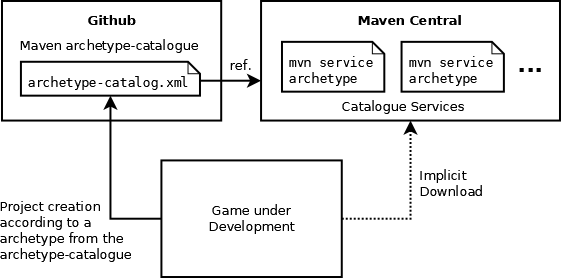
\includegraphics[width=12cm]{images/architecture/ServiceCatalogue}
	\caption{Integration of the service catalogue in \og{} development.}
	\label{fig:service_catalogue}
\end{figure}

The mostly used \ms{} of the service catalogue is the ``Hello World''
service which provides the means of bringing up a new \ms{} quickly.

\subsubsection{Consistency Requirements}

Consistency is a big concern in any distributed application and \ogs{} are no
exception. Consistency requirements for \ogs{} has already been researched in
project thesis one \todo{5.4 Non-functional requirements} and have been further
examined in this semester.

For \ogs{} consistency requirements can be categorized into strong consistency
for sensitive data like account or payment information and eventual consistency
for all other non critical game data. 

The final solution to consistency in MicroNet emphasises exactly this two
requirements. For transaction which require strong consistency it is aways
necessary that one single \ms{} maintains the overall control over the complete
transaction. This service then must use the underlying relational database to
make the transaction ACID by using the two phase commit protocol offered by the
database which is ProstgreSQL for MicroNet. This approach is mainly chosen due
to the reason that ACID transaction using eventual consistency are hard to get
right and therefore are error-prone \cite{zhang2011transaction},
\cite{zhang2008persistence}, and \cite{pardon2014atomic}.

For best effort consistency requirements eventual consistency is a solution that
has proven to work \cite{graham2016distributed_transactions}. Eventual
consistency emphasis scaling and robust systems in general. The drawback is the
added effort during development to implement a eventual consistent application.

Eventual consistency in MicroNet is realized by time-outs and retries. This is
realized by using the presistence system of the message broker in conjunction
with the request response functionality offered by MicroNet messaging. \mss{}
are advised to retry a transaction for a number of times\footnote{Five retries
seemed appropriate for most requests.}. If all retries where failures the
service must persistently log the unprocessed transaction and send an
informative message to the user. Over time the number of unprocessed transaction
should decrease. Unprocessed transaction can then be examined by developers in a
batch to find flaws in the application design.
developers
